\documentclass[../Book.Stress_regulation.tex]{subfiles}
\graphicspath{{\subfix{../images/}}}
\begin{document}


\subsubsection{The Start of the Stress Reaction  ---  Seat of the Alarm Central}
Stress starts with the {sensory organs}. Endogenous\footnote{Coming from the inside} and exogenous\footnote{Coming from the outside} {sensory impulses} get registered at the receptor of the {sensory cells}.
 The sensory impulses creates an {electric impulse} in the nervous cells which transmit the information, which is called an {excitation}.
 The impressions get passed on to the {limbic system}, which {processes them} before they get transmitted to the brain.


\begin{figure}[htb]
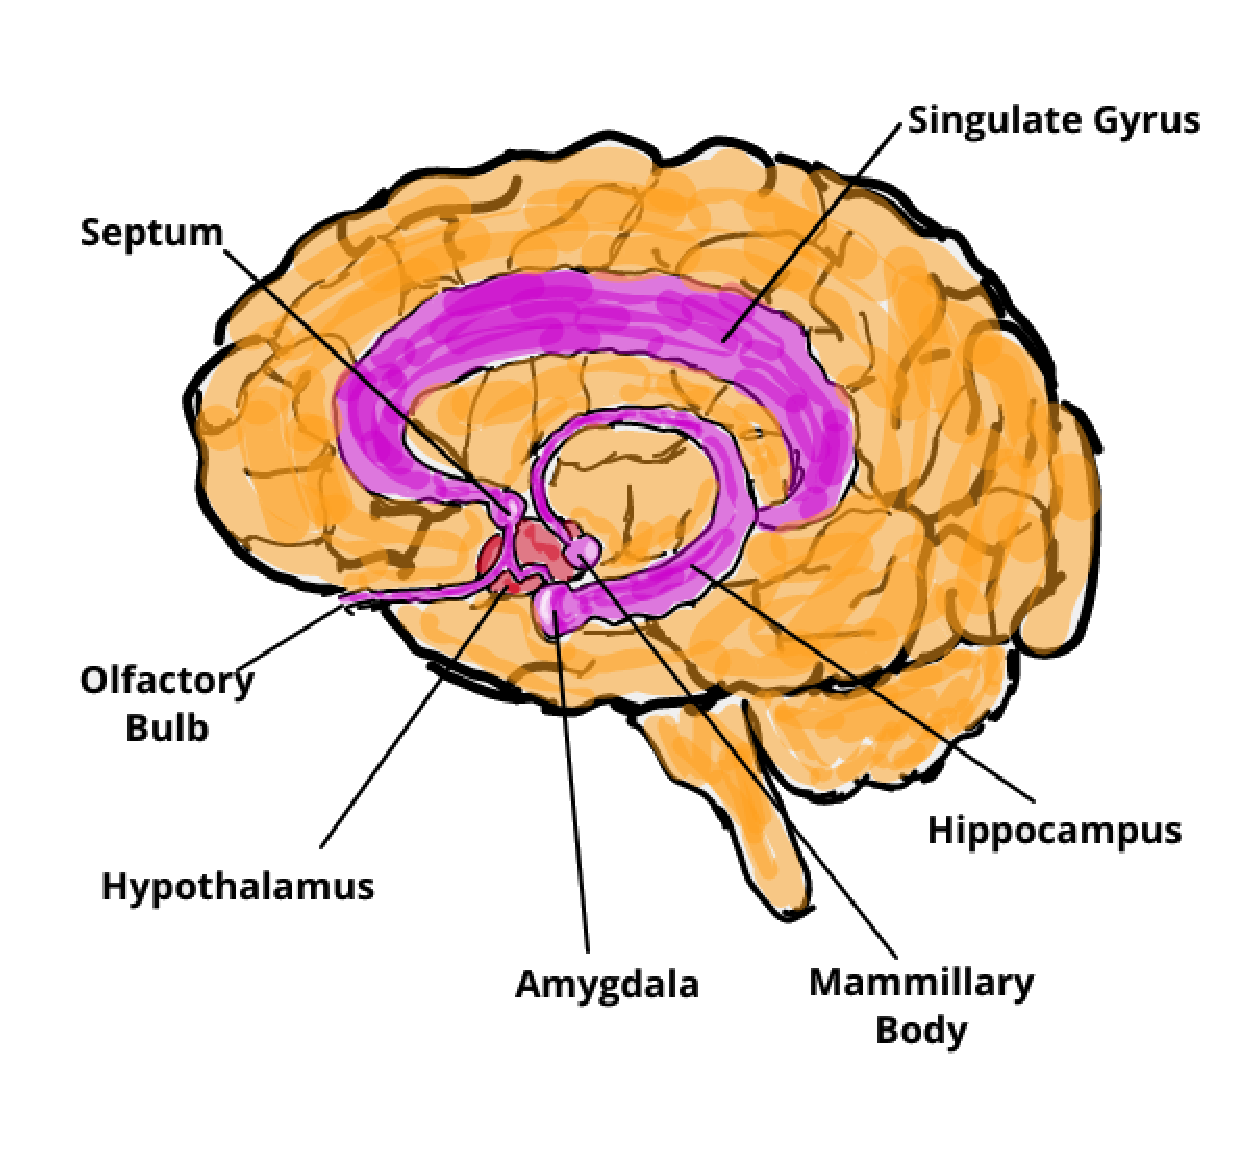
\includegraphics[width=7cm]{Limbic_System.eps}
\caption{The limbic system in the human brain.}
\end{figure}



\subsubsection{Processing in the Limbic System}

The limbic system is a {deeper lying part} of the brain, which regulates {instinctive
  reactions}\index{reaction!instinctive}, like the \emph{fight or flight} reaction in the stress situation.
Parts of this ring shaped system play a complex and important part in the {expression of drives and emotions}\index{drives}\index{emotions} and the influence of the state of the mood on the external behaviors and the memory (translated from \cite{DorlingAtlas}).
%-----------------------------------------------------------
%------------------------------------------------

The following systems get regulated in the limbic system:
\begin{enumerate}
\item {Sleep--awake state and cycle}
\item {Nutrition}
\item {Procreation}
\item {Feelings and emotions}\footnote{We distinguish between feelings and emotions. An {emotion is a reaction} to a feeling.}
\end{enumerate}


%------------------------------------------------


If one of these systems gets disturbed it will {cause a stress reaction}. Possible disturbances are sleep deprivation, eating compulsion, sexual abuse or psycho terror.
All these systems are responsible for the {alarm reaction}.

\subsubsection{Stress Regulation}


The limbic system is the {main focus of stress regulation}.
That means we watch out for a {healthy and balanced body household} in terms of\footnote{There's no such a thing as a magic pill :-) }
\begin{itemize}
\item Sleeping and waking times
\item Nutrition
\item Sexuality % xxx comment out for kids.
\item Landscape of feelings
\item Exchange of emotions
\end{itemize}



\end{document}